\documentclass{article}

\usepackage{fullpage}
\usepackage{url}
\usepackage{bbm}
\usepackage{graphicx}
\usepackage{amsmath}
\usepackage{physics}
\usepackage{mathtools}
\usepackage{bbold}
\usepackage{slashed}
\usepackage{pxfonts}
\usepackage{multicol}
\usepackage{mathptmx}
\usepackage{simplewick}
\usepackage{placeins}

\usepackage{lmodern}
\usepackage[T1]{fontenc}
\usepackage[fontsize=13.5pt]{fontsize}

\DeclareMathOperator{\erfi}{erfi}
\newcommand{\R}{\ensuremath{\mathbb{R}}}
\newcommand{\C}{\ensuremath{\mathbb{C}}}

\title{Quantum Field Theory I Excercise 8}
\author{Idan Stark}
\date{\today}

\begin{document}
\maketitle

\section{A fixed point in the $\phi^3$ theory}
\subsection{The linear term of the Wilsonian beta function of $g$}
For any theory in $d$ dimensions, since the kinetic term must have mass dimension $d$, the dimension of $\phi$ must be:
\begin{equation}
    2[\partial_\mu\phi] = d, [\partial_\mu] = 1 \rightarrow [\phi] = \frac{d - 2}{2}
\end{equation}
This means that the mass dimension of $g$ is:
\begin{equation}
    [g] = d - 3[\phi] = d - 3\frac{d - 2}{2} = \frac{6 - d}{2}
\end{equation}
Now, since $m = g = 0$ is a fixed point of the theory, the linear terms of the Wilsonian beta for $g$ is actually the Wilsonian gamma $\gamma^g$, which is, as we saw, the mass dimension of $g$:
\begin{equation}
    \gamma^g = \frac{6 - d}{2}
\end{equation}
\subsection{Perturbation around $d = 6$}
We can thus write the Wilsonian beta function as:
\begin{equation}
    \beta_{Wil}^g = \gamma^g_g g + \mathcal{O}(g^3)
\end{equation}
Where we stick to odd powers of $g$ from the antisymmetry of the theory. Setting the dimension to be $d = 6 - \epsilon$, we can write it as:
\begin{equation}
    \beta_{Wil}^g = \frac{\epsilon}{2} g + \mathcal{O}(g^3)
\end{equation}
\subsubsection{The fixed point}
Perturbing in $\epsilon$ and $g$, we can write this as:
\begin{equation}
    \beta_{Wil}^g = \frac{\epsilon}{2} g + \mathcal{O}(g^3)
\end{equation}
Now, we know that for $d = 6$, meaning $\epsilon = 0$, we get:
\begin{equation}
    \beta_{Wil}^g = -\frac{3}{4(4\pi)^3} g^3 + \mathcal{O}(g^5)
\end{equation}
So, for non-zero $\epsilon$ that is still small enough for the approximation to hold, we can write:
\begin{equation}
    \beta_{Wil}^g = \frac{\epsilon}{2} g -\frac{3}{4(4\pi)^3} g^3 + \mathcal{O}(g^5)
\end{equation}
Looking for a non trivial fixed point $\beta_{Wil}^g(g^*) = 0$ we get:
\begin{equation}
    g^* = \pm\sqrt{\frac{2(4\pi)^3}{3}\epsilon}
\end{equation}
Which means that for small enough positive values of $\epsilon$ there is a non-trivial fixed point.

\subsection{The dimension of $\phi^3$ operator}
The anamolous dimension of $\phi^3$ is then the linear term of the beta function, which can be approximated to the derivative of the beta function at this fixed point:
\begin{equation}
    \gamma_{Wil}^{g} = \frac{d}{dg}\beta_{Wil}^{g}\Big|_{g^*} = \frac{\epsilon}{2} - \frac{9}{4(4\pi)^3} {g^*}^2  = \frac{\epsilon}{2} - \frac{9}{4(4\pi)^3} \frac{2(4\pi)^3}{3}\epsilon = -\epsilon
\end{equation}
So, the scaling dimension of $\phi^3$ is:
\begin{equation}
    \Delta_{\phi^3} = d + \gamma_{Wil}^{g} = 6 - 2\epsilon
\end{equation}
Now, comparing this to $d = 6 - \epsilon$, we get that for positive $\epsilon$ for which there is a fixed point:
\begin{equation}
    \Delta_{\phi^3} = 6 - 2\epsilon < 6 - \epsilon = d
\end{equation}
So, $\Delta_{\phi^3} < d$. This means that as we go to lower and lower energies, the operator will scale up. This makes it a relevant operator.
\newline
Looking around the fixed point, the beta function has a negative derivative:
\begin{equation}
    \beta_{Wil}^g \approx -\epsilon (g - g^*)
\end{equation}
This means that the flow pulls towards the fixed point.

\section{The exact renormalization group equation}
The exact renormalization group equation is:
\begin{equation}
\begin{gathered}
    \frac{dg_n(p_1, \dots, p_n)}{d\Lambda} = \frac{1}{2} \int \frac{d^d p}{(2\pi)^d} \sum_{k, \{n\}} g_{k+1} (p_1, \dots, p_{k}, p) \times \\ \times (2\pi)^d \delta^{(d)}\left(\sum_i p_i + p\right) \frac{\partial K^{-1}(p^2)}{\partial\Lambda} g_{n-k+1} (p_{k+1}, \dots, p_n, -p) - \\ -
    \frac{1}{2} \int \frac{d^d p}{(2\pi)^d} \frac{\partial K^{-1}(p^2)}{\partial\Lambda} g_{n+2} (p_1, \dots, p_{n}, p, -p)
\end{gathered}
\end{equation}
For our theory with
\begin{equation}
    g_n(\Lambda_0) = \begin{cases}
        g & n = 3 \\ 0 & else
    \end{cases}
\end{equation}
\subsection{Leading order couplings}
Starting to generate $g_n$ order by order, in first order og $g$ we have the terms that are generated by the linear term in the above equation. This required
\begin{equation}
    g_{n+2} = g_3 \rightarrow n = 1
\end{equation}
But since $\langle \phi \rangle = 0$, then $g_1 = 0$ in all orders. Next order is the quadratic term, requiring:
\begin{equation}
    g_{k + 1} = g_{n - k + 1} = 3 \rightarrow n = 4, k = 2
\end{equation}
So, in leading order $g_4$ is generated. Pluggin this in gives:
\begin{equation}
    \frac{dg_4(p_1, \dots, p_4)}{d\Lambda} = g^2 \frac{\partial K^{-1}\left(\left(\sum_i p_i\right)^2\right)}{\partial\Lambda}
\end{equation}
This fits the flow of how two 3 point vertices merge to create a single 4 point vertex, where $\sum_i p_i$ is the sum of incoming momenta.
\begin{figure}[!htbp]
    \centering
    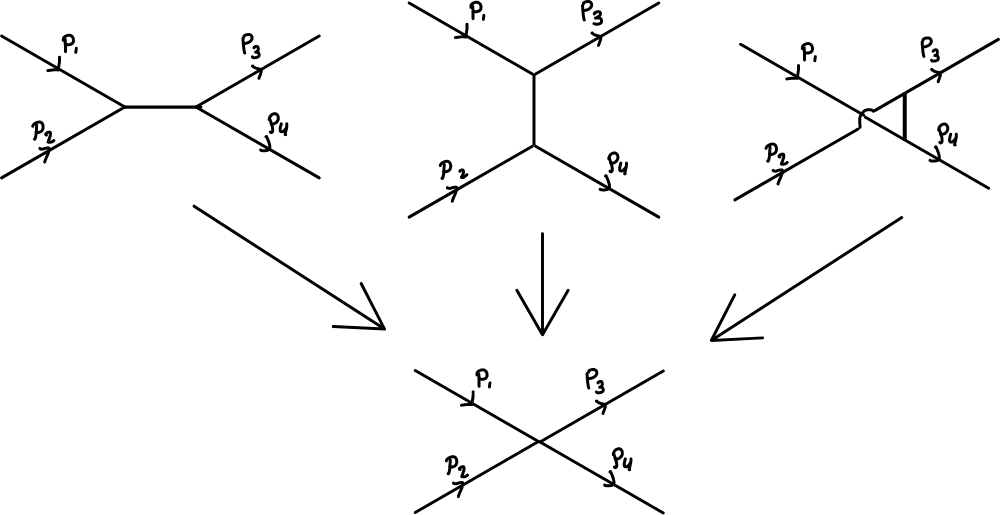
\includegraphics[width=0.5\textwidth]{figures/Notewise-Untitled 2026-01-18-20260626182718.png}
    \caption{The RG flow of three point vertices to four point vertices. The three channels, s, t, u, all flow to a single four point vertex.}
\end{figure}
Integrating:
\begin{equation}
    g_4(p_1, \dots, p_4) = g^2 K^{-1}\left(\left(\sum_i p_i\right)^2\right)
\end{equation}
Where we used $g_4(\Lambda_0) = 0$, and the sum $\sum_i p_i$ again matches the sum of incoming momenta. There are three contributing diagrams, for the three channels $s, t, u$. So, the total $g_4$ is:
\begin{equation}
    g_4(p_1, \dots, p_4) = g^2 \left[K^{-1}(s) + K^{-1}(t) + K^{-1}(u)\right]
\end{equation}
\subsection{The sharp cutoff approximation}
Using
\begin{equation}
    K^{-1}(p^2, \Lambda^2) = \frac{1}{p^2}\Theta(\Lambda^2 - p^2)
\end{equation}
Since:
\begin{equation}
    \frac{\partial K^{-1}(p^2)}{\partial\Lambda} = \frac{d\Lambda^2}{d\Lambda}\frac{\partial K^{-1}(p^2)}{\partial\Lambda^2} = \frac{2\Lambda}{p^2}\delta(\Lambda^2 - p^2) = \frac{\delta(\Lambda - p) + \delta(\Lambda + p)}{p^2}
\end{equation}
We get:
\begin{equation}
    \frac{dg_4(p_1, \dots, p_4)}{d\Lambda} = g^2 \frac{\delta(\Lambda - \sum_i p_i) + \delta(\Lambda + \sum_i p_i)}{\left(\sum_i p_i\right)^2}
\end{equation}
and since $\Lambda > 0$ only one of the delta functions will be non-zero, resulting in:
\begin{equation}
    g_4(p_1, \dots, p_4) = g^2 \left[s^{-1} + t^{-1} + u^{-1}\right]
\end{equation}
Now, the other coupling generated by the flow in order $g^2$, is the coupling that is generated linearly from $g_4$, which is the $g_2$ coupling:
\begin{equation}
    \frac{dg_2(p_1, p_2)}{d\Lambda} = - \frac{1}{2} \int \frac{d^6 p}{(2\pi)^6} \frac{\partial K^{-1}(p^2)}{\partial\Lambda} g_{4} (p_1, p_2, p, -p)
\end{equation}
Plugging in the sharp cutoff $K^{-1}$:
\begin{equation}
    \frac{dg_2(p_1, p_2)}{d\Lambda} = - \frac{1}{2} \int \frac{d^6 p}{(2\pi)^6} \frac{\delta(\Lambda - p) + \delta(\Lambda + p)}{p^2} g_{4} (p_1, p_2, p, -p)
\end{equation}
Now, from the three channels we get
\begin{equation}
    s = \left(p_1 + p_2\right)^2
    \qquad
    t = \left(p_1 + p\right)^2
    \qquad
    u = \left(p_1 - p\right)^2
\end{equation}
Using $d^6p = \pi^3 p^5 dp$ and then the radial integation variable $p \ge 0$ gives:
\begin{equation}
    \frac{dg_2(p_1, p_2)}{d\Lambda} = - \frac{g^2}{2} \int \frac{\pi^3 p^3 dp}{(2\pi)^6}\delta(\Lambda - p)\left[\frac{1}{\left(p_1 + p_2\right)^2} + \frac{1}{\left(p_1 + p\right)^2} + \frac{1}{\left(p_1 - p\right)^2}\right]
\end{equation}
\begin{equation}
    \frac{dg_2(p_1, p_2)}{d\Lambda} = - \frac{\pi^3}{(2\pi)^6}\frac{g^2 \Lambda^3}{2} \left[\frac{1}{\left(p_1 + p_2\right)^2} + \frac{1}{\left(p_1 + \Lambda\right)^2} + \frac{1}{\left(p_1 - \Lambda\right)^2}\right]
\end{equation}
The $g_2$ flow generated by $g_4$ is the flow of a single four point function with a loop.
\begin{figure}[!htbp]
    \centering
    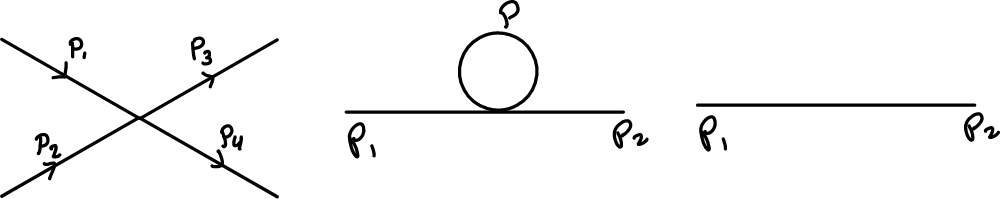
\includegraphics[width=0.5\textwidth]{figures/Notewise-Untitled 2026-01-18-20260626183730.png}
    \caption{The RG flow of four point vertex to a two point vertex passes through a loop.}
\end{figure}
\subsection{The flow from $g^3$ to a single vertex}
Starting from the triangle loop diagram we saw in tutorial, the flow will start integrating over momentum in a way that will eventuall merge two vertices to create a single four point vertex, leaving the third three point vertex alone. Then, the last vertex is also merged to create a five point vertex, before the remaining loop is integrated and the result is back to a 3 point vertex. This can be viewed in figure \ref{fig:last}
\begin{figure}[!htbp]
    \centering
    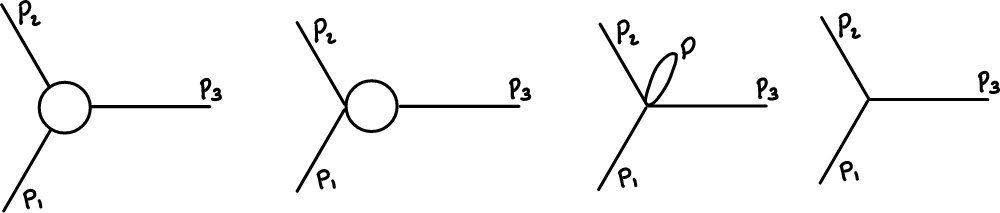
\includegraphics[width=0.5\textwidth]{figures/Notewise-Untitled 2026-01-18-20260626183035.png}
    \caption{The RG flow from the triangle loop diagram to a single 3 point vertex passing through a four point vertex and a five point vertex.}
    \label{fig:last}
\end{figure}
\newline
This can also be viewed from the RG flow. $g_3$ will generate $g_4$ from the quadratic term, which in turn will generate $g_2$ from the linear term and $g_5$ from the quadratic term. $g_5$ then again generates $g_3$ from the linear term.
\end{document}
